%!TEX program = pdflatex
\documentclass[a4paper]{article}
\title{\textbf{Homework 8}}
\author{Wendi Chen}
\date{}
\usepackage{listings}
\usepackage{graphicx} 
\usepackage{indentfirst} 
\usepackage{algorithm}
\usepackage{algorithmicx}
\usepackage{algpseudocode}
\usepackage{amsmath}
\newtheorem{proof}{Proof}[section]
\usepackage{algorithm,algpseudocode,float}
\usepackage{lipsum}
\usepackage{tikz}
\lstset{
 columns=fixed,       
 numbers=left,                                        % 在左侧显示行号
 numberstyle=\tiny\color{gray},                       % 设定行号格式
 frame=none,                                          % 不显示背景边框
 backgroundcolor=\color[RGB]{245,245,244},            % 设定背景颜色
 keywordstyle=\color[RGB]{40,40,255},                 % 设定关键字颜色
 numberstyle=\footnotesize\color{darkgray},           
 commentstyle=\it\color[RGB]{0,96,96},                % 设置代码注释的格式
 stringstyle=\rmfamily\slshape\color[RGB]{128,0,0},   % 设置字符串格式
 showstringspaces=false,                              % 不显示字符串中的空格
 language=python,                                        % 设置语言
}
\makeatletter
\newenvironment{breakablealgorithm}
  {% \begin{breakablealgorithm}
   \begin{center}
     \refstepcounter{algorithm}% New algorithm
     \hrule height.8pt depth0pt \kern2pt% \@fs@pre for \@fs@ruled
     \renewcommand{\caption}[2][\relax]{% Make a new \caption
       {\raggedright\textbf{\ALG@name~\thealgorithm} ##2\par}%
       \ifx\relax##1\relax % #1 is \relax
         \addcontentsline{loa}{algorithm}{\protect\numberline{\thealgorithm}##2}%
       \else % #1 is not \relax
         \addcontentsline{loa}{algorithm}{\protect\numberline{\thealgorithm}##1}%
       \fi
       \kern2pt\hrule\kern2pt
     }
  }{% \end{breakablealgorithm}
     \kern2pt\hrule\relax% \@fs@post for \@fs@ruled
   \end{center}
  }
\makeatother
\begin{document}
\maketitle

\section{Q1}
\subsection{Is deeper better in Deep Learning?}
The answer is \textbf{Yes}. 
According to Universality Theorom, any continuous function can be realized by a 
network with one hidden layer if enough hidden neurons is given. 
However, the number of the neurons is limited, so how we arrange them matters. 
According to the study mentioned in the keynotes\footnote{Seide, Frank, Gang Li, and Dong Yu. 
"Conversational Speech Transcription Using Context-Dependent Deep Neural Networks." Interspeech. 2011.}, 
a shallow 1-hidden-layer network using the same number of parameters as the 
7-hidden-layer one leads to five percentage points worse word-error rate.
Besides, a deeper network does better in modularization.
That means the network can have some "basic classifiers" which works as module for the following classifiers 
so that the classifiers can be trained by little data.
\subsection{What parameters/designs/structures should be care-
fully concerned to obtain high performance in Deep Learning?}
\begin{itemize}
\item connection between layers
\item number of neurons in each layer \& number of layers
\item activation function \& loss function
\item optimization method(gradient descent, SGD, momentum, etc.)
\item learning rate/adaptive learning rate
\item batch division
\item training times
\item dropout
\end{itemize}

\newpage
\section{Q2}
The structure of the Neural Network is shown as follow. 
The network uses ReLU as the activation function, SGD as optimization method and L1-loss as loss function.

~\\
\tikzset{%
  every neuron/.style={
    circle,
    draw,
    minimum size=1cm
  },
  neuron missing/.style={
    draw=none, 
    scale=4,
    text height=0.333cm,
    execute at begin node=\color{black}$\vdots$
  },
}

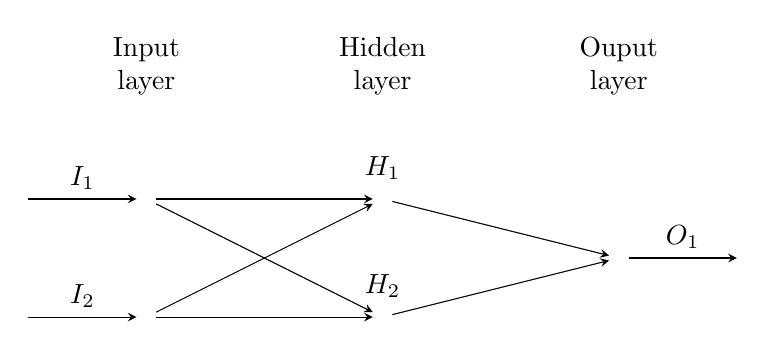
\begin{tikzpicture}[x=1.5cm, y=1.5cm, >=stealth]

\foreach \m/\l [count=\y] in {1,2}
  \node [every neuron/.try, neuron \m/.try] (input-\m) at (0,2-\y) {};

\foreach \m [count=\y] in {1,2}
  \node [every neuron/.try, neuron \m/.try ] (hidden-\m) at (2,2-\y) {};

\foreach \m [count=\y] in {1}
  \node [every neuron/.try, neuron \m/.try ] (output-\m) at (4,1.5-\y) {};

\foreach \l [count=\i] in {1,2}
  \draw [<-] (input-\i) -- ++(-1,0)
    node [above, midway] {$I_\l$};

\foreach \l [count=\i] in {1,2}
  \node [above] at (hidden-\i.north) {$H_\l$};

\foreach \l [count=\i] in {1}
  \draw [->] (output-\i) -- ++(1,0)
    node [above, midway] {$O_\l$};

\foreach \i in {1,2}
  \foreach \j in {1,2}
    \draw [->] (input-\i) -- (hidden-\j);

\foreach \i in {1,2}
  \foreach \j in {1}
    \draw [->] (hidden-\i) -- (output-\j);

\foreach \l [count=\x from 0] in {Input, Hidden, Ouput}
  \node [align=center, above] at (\x*2,1.8) {\l \\ layer};

\end{tikzpicture}

~\\

I have implemented it in PyTorch.
\begin{lstlisting}
import torch
import torch.nn as nn
import numpy as np

#data
x = np.array([[0,0],[1,1],[1,0],[0,1]])
y = np.array([[0],[0],[1],[1]])
x = torch.Tensor(x).float()
y = torch.Tensor(y).float()

#network design
class XOR(nn.Module):
    def __init__(self):
        super(XOR,self).__init__()
        self.input_layer = nn.Linear(2,2)
        self.relu = nn.ReLU()
        self.output_layer = nn.Linear(2,1)

    def forward(self,x):
        o1 = self.relu(self.input_layer(x))
        o2 = self.relu(self.output_layer(o1))
        return o2

xor = XOR()
loss_function = nn.L1Loss()
optimizer = torch.optim.SGD(xor.parameters(), 
            lr=1e-3, momentum=0.9)


#train
for epoch in range(5000):
    out = xor(x)
    loss = loss_function(out,y)
    optimizer.zero_grad()
    loss.backward()
    optimizer.step()

#test
out = xor(x)
print(out)
  \end{lstlisting}
As the test result listed below, 
the training result is not bad.
\begin{lstlisting}
  tensor([[0.0000],
        [0.0000],
        [1.0005],
        [0.9990]], grad_fn=<ReluBackward0>)
\end{lstlisting}

\section{Q3}
For question \textbf{a}, $y_1 = 4$ and $y_2 = 0$.

For question \textbf{b}, $y_1 = 0$ and $y_2 = 1.125$.
\end{document}


